%%%%%%%%%%%%%%%%%%%%%%%%%%%%%%%%%%%%%%%%%%%%%%
%                insertmeeting
% 1) Title (something creative & funny?)
% 2) Date (MM/DD/YYYY)
% 3) Location (ex. Hagerty High School)
% 4) People/Committees Present 
% 5) Picture 
% 6) Start Time & Stop Time (ex. 12:30AM to 4:30PM)
%%%%%%%%%%%%%%%%%%%%%%%%%%%%%%%%%%%%%%%%%%%%%%
\insertmeeting 
	{OpenCV Eyes} 
	{01/21/22} 
	{Hagerty High School}
	{Clayton, Falon, James, Jensen, Nathan, Ritam, Rose, Samantha}
	{Images/RobotPics/robot.jpg}
	{2:30 - 4:30}
	
\hhscommittee{Software}
\noindent\hfil\rule{\textwidth}{.4pt}\hfil
\subsubsection*{Goals}
\begin{itemize}
    \item Start a new OpenCV pipeline to identify the carousel post 

\end{itemize} 

\noindent\hfil\rule{\textwidth}{.4pt}\hfil

\subsubsection*{Accomplishments}
In Tele-Op, we have experienced difficulty navigating accurately to the carousel. One solution we decided to explore today was finding the colored pole of the carousel using OpenCV, and receiving positional data from that. To accomplish this, we used a program called GRIP. The software allowed us to test various configurations of image manipulation and computer vision techniques to refine the input. We used a picture of the carousel taken by a phone as a test image. At first, we tried to grayscale the image and use an adaptive threshold. However, the software was unable to differentiate the colored pole from the background due to the shadow from the carousel. We then attempted to improve the quality of the image through erosions and dilations. However, this method still suffered from the shadow on the carousel. So, we decided to switch to using an HSV threshold, combined with the erosions and dilations. This produced a usable image. In the future, we have to focus on refining the HSV threshold of the pipeline and calculating the correct contour. We can do this by drawing rectangles on the image and saving them into the control hub. 

\begin{figure}[htp]
\centering
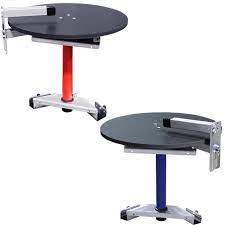
\includegraphics[width=0.95\textwidth, angle=0]{Meetings/January/01-21-22/1.21.22 carousel posts - James Hu.jpeg}
\caption{Images we used while creating the pipeline}
\label{fig:012122_1}
\end{figure}


\whatsnext{
\begin{itemize}
    \item Continue to refine the pipeline and integrate into tele-op. 
\end{itemize} 
}

